\begin{figure*}[h]                                                           
 
\includegraphics[width=\linewidth]{./media/images/chess.jpg}%
  \scriptsize{\textsc{\\we now have} effectively limitless capability to build
    dynamic, immersive world models.}
  \label{fig:editorial}%                                                 
\end{figure*}                                                                
\begin{quotation} 
\noindent\color{Sepia}{{\textit{\textbf{“Any sufficiently advanced technology is indistinguishable from magic.”
 }}}}\\[.5mm]
   \hfill\color{Sepia}{\small{\textendash Clarke's Law}}
\end{quotation} 
%\begin{abstract}
%\textbf{\emph{“In the beginning the Universe was created. This has made a lot of people very angry and been widely regarded as a bad move.”  \\ \\--- Douglas Adams}}
%\end{abstract}
\newpage
\marginnote{Editor's note: margin notes in red signify links pointing to sites of reference}[2em]
\lettrine[lines=3]{\color{BrickRed}I}{\enspace n} 1997 champion Gary Kasparov
lost to \textsc{ibm}'s ``Deep Blue'' supercomputer in a highly publicized
match.\reversemarginpar\marginnote{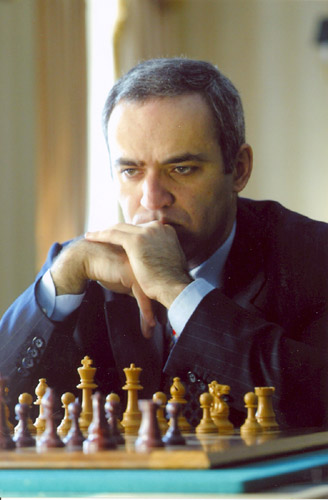
\includegraphics[width=\linewidth]{./media/images/gary}
  \href{https://www.youtube.com/watch?v=NJarxpYyoFI}{Gary Kasparov's match with
    ``Deep Blue'' was highly publicized and carried philisophical
    implications}}\label{img:kasparov}\pagenote[Page \pageref{img:kasparov}
World Champion Gary Kasparov]{Gary Kasparov image Copyright 2007, S.M.S.I., Inc.
  – Owen Williams, \href{http://www.kasparovagent.com/photo_gallery.php}{The
    Kasparov Agency},
  \href{https://commons.wikimedia.org/w/index.php?curid=4507357}{CC BY-SA 3.0}}
In 2011, \textsc{ibm}'s purpose\textendash built computer, named Watson and
developed to compete on the quiz show \textit{Jeopardy!}, prevailed over
legendary champions Brad Rutter and Ken Jennings to win first place and take the
\$1 million prize. In 2016, Google's
AlphaGo\normalmarginpar\marginnote{\href{https://en.wikipedia.org/wiki/AlphaGo}{Wikipedia:
    AlphaGo}}[-1em] computer program defeated the Go world champion, Lee Sedol, in a
five\textendash game professional match.
\marginnote{%\vspace{-6em}
  \href{https://www.youtube.com/watch?v=P18EdAKuC1U}{Watson prevailed over
    legendary champions Brad Rutter and Ken Jennings to win first place and the \$1 million prize}}\label{link:watson}In each case, the computer scientists is met with skepticism. In each case, the
dedicated technologists proved the skeptics wrong. At the crest of each new
achievement, philosophers asked the next logical questions thus restarting the cycle of discovery and progress.

By leveraging big data, artificial neural networks, and natural language
processing we can continue to explore new horizons.

%\marginnote{
%  {\href{https://en.wikipedia.org/wiki/Go_(game)}{Go}
%}

\section{socratic method of immersion}
What makes games so engaging is their way of pushing our human experience.
\marginnote{
  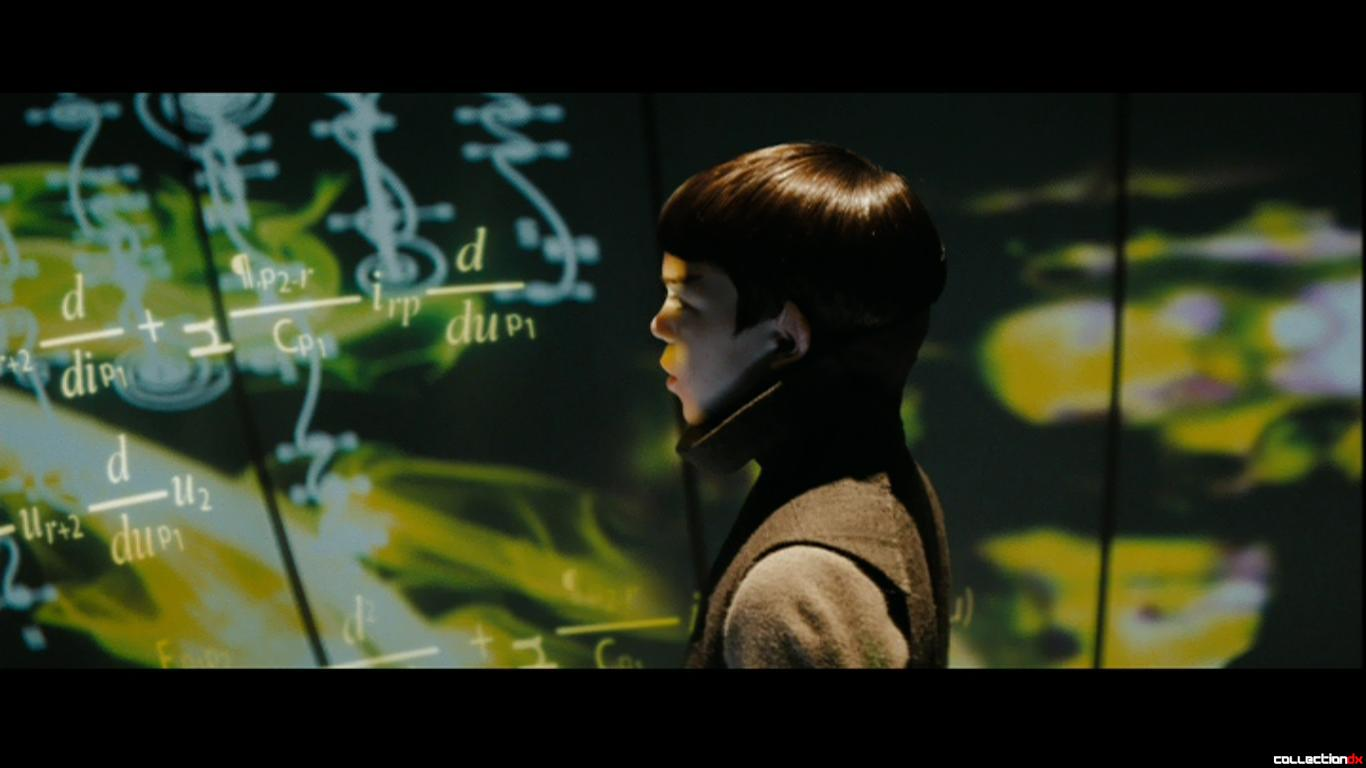
\includegraphics[width=\linewidth]{./media/images/spock}
  Spock's formative schooling in ``Star Trek'' depicts
      hyper\textendash interactive
    education
}\label{img:spock}
They patiently and quietly ask us to tackle tough problems on our own. They make
us search our knowledge and intuition. The quiet rewards for our struggles are
those moments in our lives when we feel like we accomplished the before
unattainable. Challenging, positive interactivity engages our souls. It makes us, ``better than yesterday.''

If engagement is a significant factor in 
quantifiably productive\marginnote{\href{https://www.sciencemag.org/news/2014/05/lectures-arent-just-boring-theyre-ineffective-too-study-finds}{Lectures aren't just boring they're ineffective too, study finds}}[2em] experiences then it stands to reason that a kind of Socratic ``give and take'' yields higher satisfaction and knowledge retention.
Interlocutors, like Kasparov or Sedol, query their environment. It replies with
meaningful responses. Similarly, the interactive question\textendash
and\textendash answer format of \textit{Jeopardy!} offers a distilled form of
mutual concession; it's mechanics lay bare the underpinnings of good Interactive
Fiction. When we ask intelligent questions of our world we expect fulfilling,
logical answers. When we get meaningful answers, we treasure that meaning like a prized possession.

\subsection{make it good}
\noindent Chris Crawford describes the value and nature of good
interactivity:
\begin{quote}
\marginnote{\href{https://youtu.be/3BPERIDSxKo?t=868}{Chris Crawford expresses
    the nauture and value of interactivity in an interview for ``Get Lamp''}}[2em]
The value of interactivity arises from the way the human mind responds to it.
The human mind is not a passive receptacle\textemdash it's an active agent. We don't learn
by sitting on our fat butts and listening or watching or hearing or passively
receiving information. We learn by reaching out to the world and messing around
with it with our fingers.
\end{quote}

\noindent Experience and research shows that high\textendash quality interactivity enhances the participants' satisfaction and
persistence with the content. \marginnote{\href{http://jolt.merlot.org/vol10no2/croxton_0614.pdf}{The Role of Interactivity in Student Satisfaction and Persistence in Online Learning}}
But the interactive environment must remain focused, substantively complete, and\textemdash most of
all\textemdash engaging. Understanding the power and fragility of interactive models
means understanding that the construction of solid frameworks is necessary from
the very start of our work.

Complete interactivity \textit{prima facie} implies that we need to
build a complete world model. By our ``completeness theory,'' the reader must be
able to rob a bank in a work of interactive
romance comedy, or else the system cannot provide plausible engagement.
Fortunately, experience  
suggests that total world modeling is not necessary for immersion. We find our
saving grace in the capability of our minds to suspend disbelief for the purpose
of enjoying the experience. 

In an interview for \textit{Get Lamp}, Crawford addresses\label{link:extent_model} the level of detail required for our world model
to provide credible stories:
\begin{quote}
\marginnote{\href{https://youtu.be/3BPERIDSxKo?t=1604}{Chris Crawford discusses
    the extent to which a complete world model is necessary in an interview for ``Get Lamp''}}[1em]A lot of people, I think, mis\textendash understand the nature of interactivity thinking that it requires giving the player absolute freedom. That's not at all what interactivity requires. It merely requires giving the player \textit{all relevant, useful freedom}.
\end{quote}
We've seen audiences enjoy and learn
from\marginnote{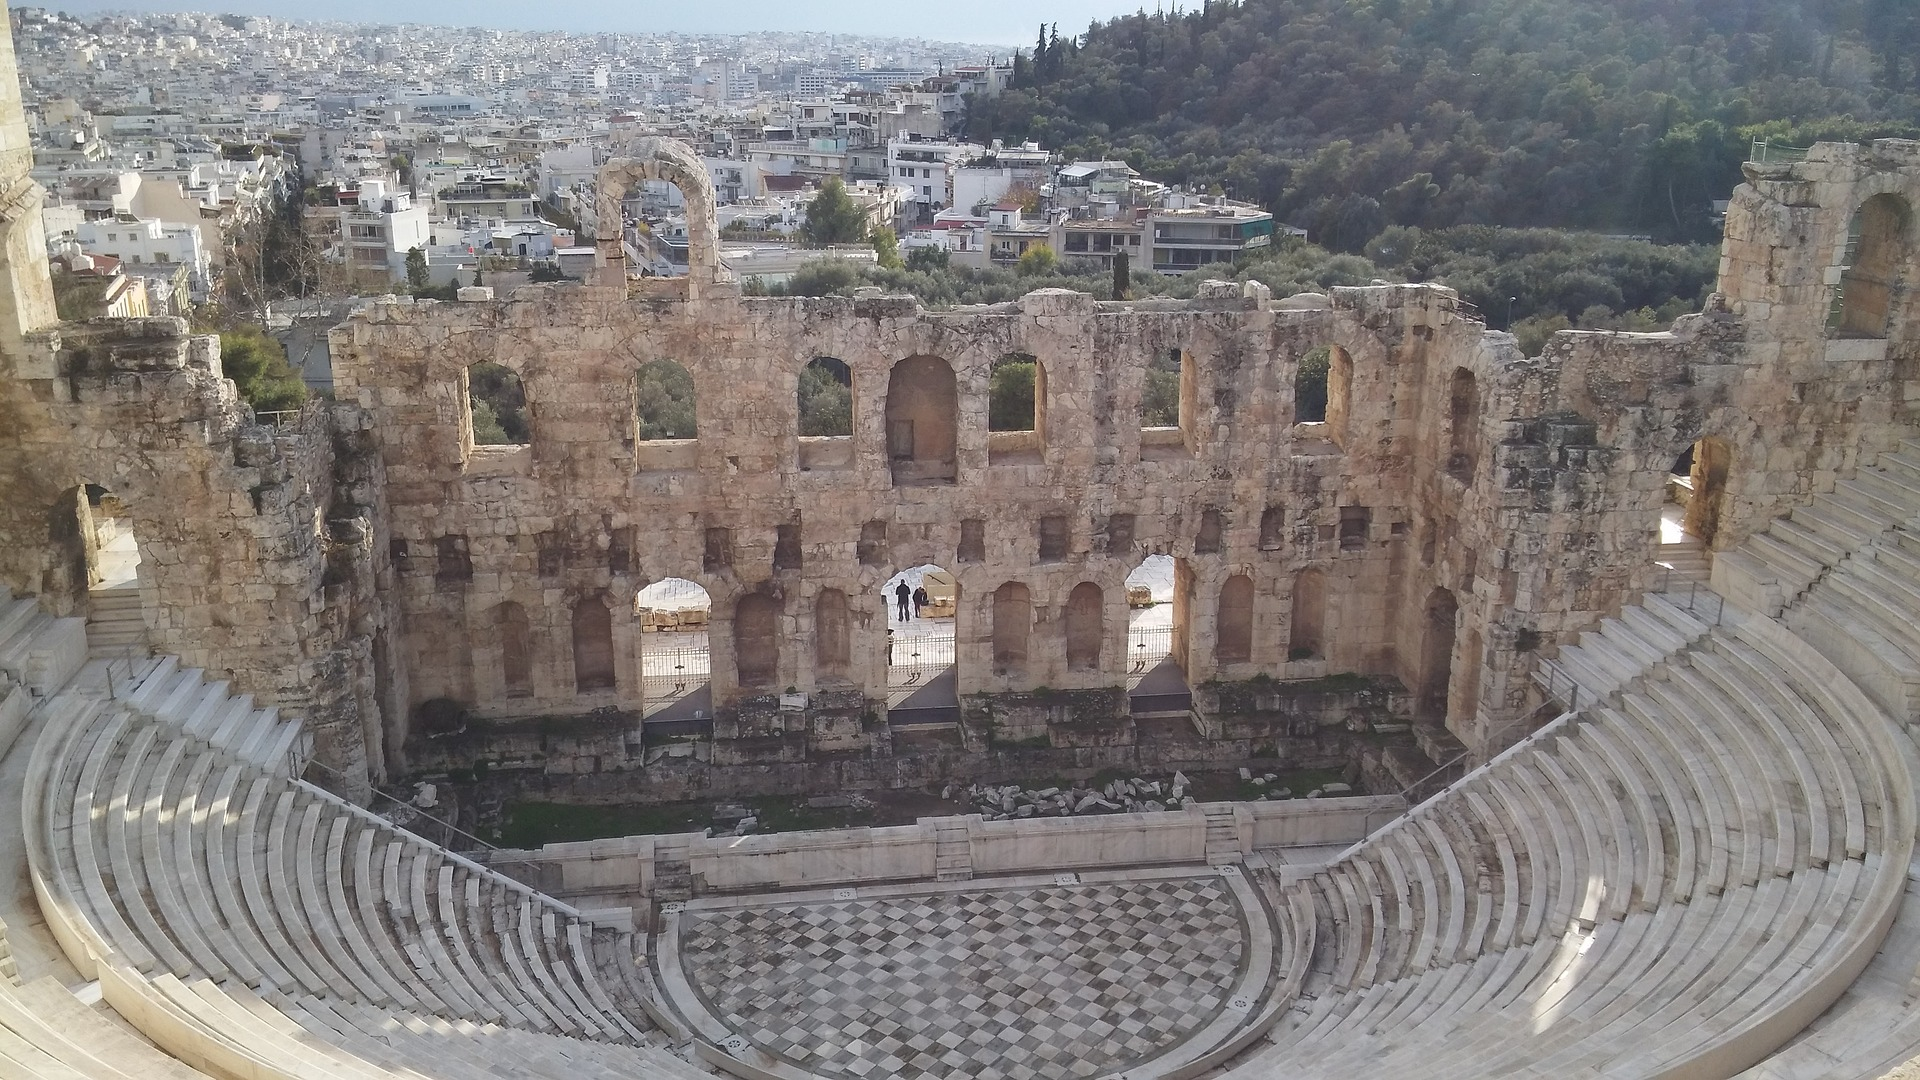
\includegraphics[width=\linewidth]{./media/images/greek_theatre}
  \tiny{\textit{Audiences consume themselves in stories while sitting on stone
      slabs through suspended disbelief}}} stories from as far back as the Greek
Tragedies, when great warriors and fair maidens entertained crowds that sat in
stadium style theaters on stone slabs. A story's efficacy doesn't come directly
from the physical setting of the audience. The theater sets the mood, while the
careful crafting of dialog, executed with superb timing, delivers the story's
impressions, which can be profound. The message speaks to us on primal levels
that
\marginnote{\href{https://greatergood.berkeley.edu/article/item/how_stories_change_brain}{Paul
    J. Zak, How Stories Change the Brain}} can be measured. Beyond the science,
writers deliver experiences by relying less on settings and more on \textit{story}.
\subsection{the struggle eternal}
Writing complete Interactive
  Fiction worlds by hand is a long, arduous process. There's no way around it. 
Aaron Reed, in an interview for \textit{Get Lamp} notes,
\begin{quote}
\marginnote{\href{https://youtu.be/LRhbcDzbGSU?t=2575}{Aaron Reed notes the
    complexities of creating a complete world model in \textsc{if}}}[2em]
As a player of Interactive Fiction, it's very easy to not appreciate the work
that went into it. You just come across one error message or one response that
the designer didn't think of and you think, ``Oh, well, forget this game.''
After you've actually gone through and had to think of all those things and code
them and write them yourself, your perspective really changes.
\end{quote}

\noindent Complete world models, on the other hand, where the Interlocutor feels confident that their
interactions will be met with meaningful responses is known to be the most
important factor in their enjoyment of Interactive Fiction. Emily Short writes
in her article, ``The Prose medium and \textsc{if}:''
    \begin{quote}
    \marginnote{\href{https://emshort.blog/how-to-play/writing-if/my-articles/the-prose-medium-and-if/}{Emily
        Short considers the reltionship between prose and parser function in, ``The Prose medium and \textsc{if}''}}[2em]
    By contrast, negative points made about \textsc{if} in the wider world (and here I draw
    from threads on \textsc{slashdot} about the yearly comp, and discussions on various
    gaming boards) often focus on the parser, not the writing, as the critical
    weakness of \textsc{if}. It is the refusal to recognize nouns mentioned in the text, the
    insistence on very particular player behavior, the guess-the-verb nonsense,
    that turns off the most people, as I observe it.
    \end{quote}
So it is that precisely what the reader finds most important to a good work of
\textsc{if} turns out to be the most burdensome for the implementer to write.
The implementer's task isn't limited simply by sheer mass of the world's
components; his undertaking is compounded in difficulty by the fact that he must
think of everything a reasonable reader will try to do in the world for any
given situation. The player's complete agency and the implementer's difficulty
furnishing his world model mix like oil and water.

\subsection{critical non\textendash acclaim}
Some argue the readers expectation of agency and the implementors burden to
achieve the goal will never resolve. They will say that there is no way an
implementor will come even close to a satisfactory world model without resorting
to trite gimmiks. Proponents of this argument point to efforts in the past, most
of which have fallen short. They will pine eloquent about the absolute
complexities of the task's implied workload and call upon the implmenter as
running a fool's errand.

To the critics I respond as Theodore ``Teddy'' Roosevelt did,
\begin{quote}
It is not the critic who counts; not the man who points out how the strong man stumbles, or where the doer of deeds could have done them better. The credit belongs to the man who is actually in the arena, whose face is marred by dust and sweat and blood; who strives valiantly; who errs, who comes short again and again, because there is no effort without error and shortcoming; but who does actually strive to do the deeds; who knows great enthusiasms, the great devotions; who spends himself in a worthy cause; who at the best knows in the end the triumph of high achievement, and who at the worst, if he fails, at least fails while daring greatly, so that his place shall never be with those cold and timid souls who neither know victory nor defeat.
\end{quote}
I argue that, given today's \textsc{if} authoring technology to works of the
past is a little like comparing the Nicéphore Niépce's first fixed image with a
camera to today's moving experiences found in modern film.

We have virtually no limit on the size and scope of our work and we can use all
available mediums in the world model through scripting hooks available with both
\textsc{tads3} and \textsc{inform 7}. I submit boldly that it ought even
be possible using projectors to let players roam around in a physical building
or geodesic dome where the rooms, using projectors, change as the story does.

\includepdf[scale=1.01]{media/images/dating_ad.pdf}

\subsection{critical constructs}
The question of creating rich, virtual experiences quickly escalates into
varying narrative techniques and structures, fluid linguistics, and other
aspects. I will
happily leave these discussions to the scholars as we focus on creating a
foundation that they may all build on. Our goal is to build an efficient and flexible framework whose capabilities enable all comers. 

The solution, whatever it may be, should answer this core question: ``How do we build
an engaging world whose dynamics deliver enriching engagement for the
audience?'' We assume no bounds and take only the requirement for verifiable
results to achieve our goal. If our work passes a literary Turing
Test\marginnote{\href{https://en.wikipedia.org/wiki/Turing_test}{Wikipedia:
    Touring Test}}, we are successful. Hopefully (and probably), we've created a
framework for others to follow and develop further. Our story's positive effect on the audience is our mission.

To date I know of no substitute for inspired creativity. There exists no
system\textemdash quantum or otherwise\textemdash that serves even as a shallow replacement
for inspiration. Our minds possess sophisticated neural methods for spotting
contrivance at a glance. We're embroiled in
an\marginnote{\href{http://theconversation.com/the-evolution-of-lying-14254}{Rob
    Brooks, The Evolution of Lying}} arms race between lying and honesty
detection that continues to this day. And so far the longevity of inspired works
shows a direct correlation with honesty; Plato's ``The Republic'' survives to this day, while last month's ``Enquirer'' headlines do not.

That is the first plank of our system's foundation: raw inspiration
space for the writers expressing their brutal honesty. There's no ``man behind the
curtain'' in our model. Just as Greek theaters made no claim to be
a of being Greco-Punic battlefields, we make no claims that our emulated world
is a complete manifestation of the real environment. ``However,'' we say, ``if you let
us, we will take you on a journey of laughter, sadness, or possibly both.
Perhaps we will make you think in ways you have never thought before. Above all, we will make you \textit{feel}.''


\subsection{nuts and bolts}

This issue of \textit{Discoverer's Digest} provides
step{\textendash}by{\textendash}step instructions to build topic modeling and natural language
processing systems that can greatly reduce the effort required to build your world and
narrative models. Building an authentic world requires an enormous amount of
writing; these techniques can assist greatly by generating ideas and taking care
of the mundane. The author may focus on \textit{story} rather than clerical
tasks and associations.

Both techniques draw (or can draw) their results from the entire collection of Wikipedia articles
(all 5.7 \emph{million} of them, in English alone). It's as if the entire collection human thought was at
your disposal to build your work of
Interactive Fiction. The result is a systematized method for creating complete,
relevant world models.

Topic modeling is a systematic way to flesh out 
areas that are related to a work's central themes\textemdash the broad areas that an
Interactive Fiction audience is likely to
explore. Topic modeling also helps generate completely new areas of reference
we often hadn't thought of.

It provides a ready\textendash made system that suggests
the most relevant topics for a query. Those topics
can be re\textendash entered into the system to provide greater depth and
generate additional detail with more
relevant topics, and so on.

The issue also discusses natural language processing, where we select a subject or
word phrase to see how it is used in context with surrounding text. It provides 
brief phrases that span multiple contexts for works of Interactive Fiction.

Both articles are somewhat technical. However, the step\textendash by\textendash
step instructions should make it easy to replicate their results; each step is
explained along the way. These articles use the \textsc{linux} operating
system but their techniques may be adapted for other operating systems.

% * We don't have issues of memory limits anymore
% * [[https://github.com/danielricks/scholar][Using linear algebra, we were able to pull affordances (relevant verbs) for nouns out of word2vec, with varying success on other parts of speech. This interface provides methods that perform those operations.]]
% ** So, with this, we feed the nouns in and get a list of relevant verbs, e.g.
% DOG: 'pet dog, kick dog, call dog, etc.'

% Look, I'm not suggesting the world will make the story--only polished work and
% rewrites will do that. But should we enslave ourselves to have to write the
% world from scratch?

% Of course, this isn't 
% This is what I hope to make a small dent toward achieving.

All in all, this issue provides foundational frameworks to build the
scope and context of your authorship quickly, assisting with contextual phrasing for each
geographic or narrative node in your story. Running your topics and phrases
through these systems will provide you with quick ``stubs'' to support 
your work. Its suggestions will provide moments where you think, ``ah, it's true that \textit{x} is related to
\textit{y}, I didn't think of that.''

I hope you enjoy this magazine. \emph{Discoverer's Digest } seeks to cover all manner of
topics related to Interactive Fiction, ranging from parser experiences to
choice\textemdash games, along with experiments in the medium (including General Artificial Intelligence) that we've not yet seen.

And please submit your news, story ideas, and comments by sending a personal email to \href{mailto:cooper@discdigest.xyz}{cooper@discdigest.xyz}. \\ \\

\noindent Happy Writing! \\ \\

\noindent \href{mailto:cooper@discdigest.xyz}{\textsc{D. Cooper Stevenson}}
